\cref{fig:lidarcurves} compares concentration inference with and without monotonicity under the same Gaussian model.
At $502.86$ meters, the ordinary posterior mean concentration reaches its minimum on the reconstruction grid at $-42.13$ nanograms per cubic meter, with pointwise $95\%$ equal-tail credible interval $(-94.27,10.00)$ and posterior probability $0.9434$ of a negative concentration.
Conditioning on monotonicity gives a mean concentration of $11.75$ nanograms per cubic meter at that distance, with corresponding interval $(1.10,31.23)$, while changing the response fit little.

\begin{figure}[H]
\centering
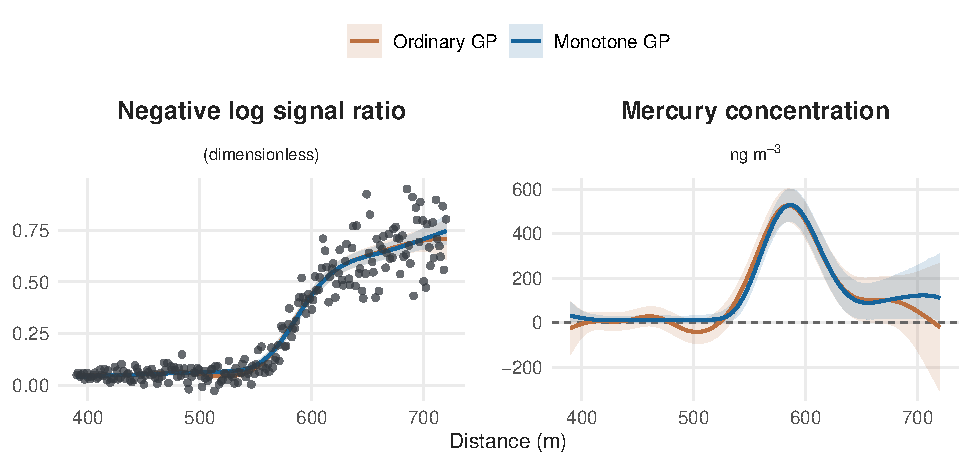
\includegraphics[width=\textwidth]{figures/lidar_monotone_fit.pdf}
\caption[Absorption and concentration inference for mercury lidar]{
The left panel shows the latent negative log signal ratio with all $221$ observations as points, and the right shows mercury concentration in nanograms per cubic meter, given under the DIAL approximation by the range derivative of the latent negative log ratio divided by $1.6\times10^{-5}$ square meters per nanogram.
Orange and blue lines denote ordinary and globally monotone posterior means, with shading for pointwise $95\%$ equal-tail latent credible intervals excluding new measurement error.
Both fits use the same rank-$128$ Mat\'{e}rn $7/2$ Gaussian regression model and range-dependent noise variances, with the monotone posterior imposing the restriction throughout $390$--$720$ meters.}
\label{fig:lidarcurves}
\end{figure}
